\documentclass[8pt, letterpaper]{article}
\usepackage[ngerman]{babel}
\usepackage{graphicx}
\usepackage[utf8]{inputenc}
\usepackage{gensymb}
\usepackage{blindtext}
\usepackage{geometry}
\usepackage{fancyhdr}
\usepackage{url}
\usepackage{seqsplit}
\usepackage{hyperref}

\graphicspath{{images/}}
\setlength{\parindent}{0cm}
\bibliographystyle{gerplain}
\geometry{letterpaper, margin=1in}
\pagestyle{fancy}

\lhead{Jakob Kirsch}
\rhead{
\includegraphics[width=3cm]{logo}}

\begin{document}

\section{Versuch 1}

\subsection{Versuchsbeschreibung}
Ein Stück Bananenschale wird vorsichtig vom Fruchtfleisch abgehoben. Diese Schale wird mehrmals mit einer Nadel oder einem Skalpell angeritzt. Die verletzten Stellen werden für fünf Minuten beobachtet. Außerdem wird die Schnittfläche des Schalenstückes betrachtet.

\subsection{Beobachtung}
Die verletzten Stellen und die direkt umliegende Schale verfärben sich nach ein paar Minuten braun.

\begin{center}
    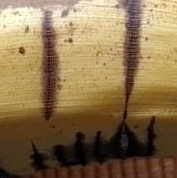
\includegraphics[width=5cm]{versuch1}
\end{center}

\section{Versuch 2}

\subsection{Versuchsbeschreibung}
Auf eine Banane wird vorsichtig ein Klebestreifen luftblasenfrei festgeklebt. Die Banane wird über Nacht im Tiefkühlfach (ca. -18 Grad Celsius) eingefroren und danach bei Zimmertemperatur mindestens vier Stunden aufgetaut.

\subsection{Beobachtung}
Die Banane verfärbt sich überall braun, wo kein Klebestreifen die Luft abhält. Zudem ist die Banane sehr weich und nass.

\begin{center}
    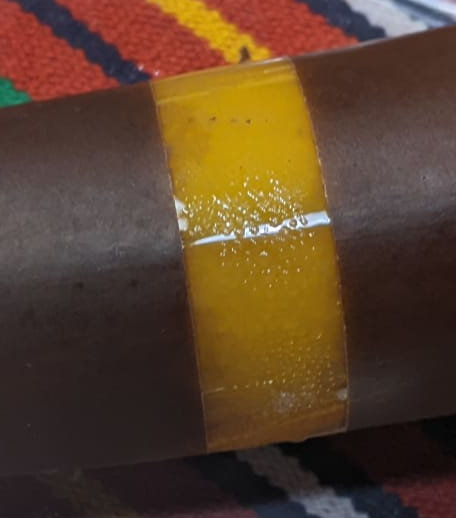
\includegraphics[width=5cm]{versuch2}
\end{center}

\section{Erklärung}
Beide Versuche lassen sich mit der Phenoloxidase erklären. Bei Versuch 1 werden die Zellen einerseits verletzt, wodurch die Phenoloxidase und die Phenole in Kontakt treten. Andererseits kommt die Phenoloxidase durch die Verletztung in Kontakt mit Sauerstoff und kann deswegen erst das Substrat oxidieren. Bei Versuch 2 hingegen werden die Zellen durch die Expansion des Wassers innerhalb der Zellen geschädigt. Die eigentliche Oxidation passiert erst nach dem Auftauen, da die Phenoloxidase bei -18 Grad Celsius so gut wie inaktiv ist (-20 Grad Celsius ist das untere Limit der Aktivität).

Der eigentliche Nutze dieses Systems liegt darin, dass das Melanin Erreger und geschädigtes Gewebe umgeben und abgrenzen kann und weitere Schäden verhindern kann. Es ist Teil des Immunsystems der Banane und wird durch die Erkennung von Erregern wie Bakterien oder Pilzen aktiviert. Dabei wird die Prophenoloxidase (proPO) zu der aktiven Phenoloxidase umgebaut, wobei weitere Teile des Immunsystems aktiviert werden. Zudem kommt die Phenoloxidase aber auch in Plastiden vor, was bei diesen Versuchen wohl eher der Fall ist.

Das am meisten oxidierte Phenol ist L-Tyrosine, welches auch eine Aminosäure ist und strukturell ein Phenylalanine mit einer Hydroxylgruppe ist.

\section{Unterdrückung}

\subsection{Einfache Lösung}
Eine offensichtliche Lösung besteht darin, die Bananen Luftdicht zu lagern. Da dies in einem Obstsalat, wie in Aufgabe 2 angegeben, schwer wird, gibt es ein paar andere Lösungen.
Man kann zum Beispiel Zitronensaft hinzugeben, da die darin enthaltene Ascorbinsäure (Vitamin C) einen pH-Wert von 1,0-2,5 hat und somit außerhalb des Bereiches der Phenoloxidase liegt. \href{https://www.ncbi.nlm.nih.gov/pmc/articles/PMC549964/}{Zudem gilt Ascorbinsäure auch als Hemmstoff}.

\subsection{Komplexere Lösung}
Die Phenoloxidase lässt sich mithilfe von Dithiothreitol oder Natriumdisulfit hemmen, wobei nur letzteres konsumiert werden sollte. \href{https://www.sciencedirect.com/science/article/abs/pii/S006526280860347X?via\%3Dihub}{Die Frage ist aber, inwiefern das gesund ist}. Ein weiterer Hemmstoff ist Cystein, eine Aminosäure.

Man kann die Bananen auch kurz stark erhitzen, um die Phenoloxidase zu denaturieren. Das geht auch mit UV- oder Gammastrahlen.

Da die Phenoloxidase Kupferionen als Cofaktor benötigt, kann man diesen mit z.B. Zitronensäure binden.

\subsection{GMO}
Eine andere Lösung besteht darin, die Bananen genetisch zu modifizieren, um die Bildung der Phenoloxidase zu unterbinden.
Die komplette mRNA der (poly) Phenoloxidase ist die folgende:

{\tiny \seqsplit{ATGGTCAGCCTTCCTAAAGCTACTCTTCCTCTCTCCTCCCTCTCCCCTCCCTCCAACTCCAACTCCAACTCCAACTCCTTTGCATGCGCCTTCCATTTTTCTTACCCTGATAGAAGACGCCATGCCCACCCCAAGATCTCATGCAAAGCTAGCGATGAGCATGAGATGACTGCAAATGCCAAGCTCGACCGCCGCGATGTGCTCGTTGGCCTCGGCGGGCTTTGTGGAGCCGCTGCCGGCCTCGGGATCGACAGTAAGGCCCTCGGAAATCCCATCCAGGCGCCTGATCTTACCAAGTGCGGCCCCGCCGATCTACCCACCGGTGCAACGCCCACCAACTGCTGCCCGCCTTATTTTCCCGACAAGAAGATTATCGATTTCAAGCGTCCGCCGAATTCGTCACCCCTCCGTGTCCGCCCGGCCGCCCACTTGGTCGACTCCGACTACCTGGACAAGTATAAGAAGGCGGTGGAGCTCATGAGGGCACTGCCGGCCGACGATCCGCGCAACTTCATGCAGCAGGCCAATGTCCACTGCGCTTACTGTGATGGCGCCTACGACCAGATCGGCTTCCCCAACCTCGAGCTCCAAGTCCACAACTCCTGGCTCTTCTTCCCTTGGCACCGCTTCTACCTCTACTTCCACGAGAGGATCCTCGGAAAGCTCATAGGCGACGACACTTTCGCCCTCCCTTTCTGGAACTGGGACGCGCCCGGCGGCATGAAGCTGCCGTCGATCTACGCCGACCCTTCGTCCTCGCTCTATGACAAGTTTCGCGACGCCAAGCACCAGCCGCCGGTCCTCGTCGACCTCGACTACAACGGAACCGACCCTAGTTTCACCGACGCAGAGCAGATCGATCAGAACCTCAAGATCATGTACCGGCAGGTGATCTCCAACGGCAAGACGCCGTTGCTCTTCTTAGGCTCGGCTTACCGTGCCGGCGACAACCCAAACCCCGGCGCGGGCTCGCTCGAGAACATACCACACGGCCCCGTCCACGGGTGGACTGGCGACAGAAGCCAACCCAATCTCGAGGACATGGGCAACTTCTACTCCGCGGGGCGCGACCCTATCTTCTTCGCCCACCATTCAAACGTCGACCGCATGTGGTACTTGTGGAAGAAGCTCGGCGGGAAGCATCAGGACTTTAACGATAAGGACTGGCTCAACACCACCTTCCTCTTCTACGACGAGAATGCTGACTTAGTTCGAGTCACCCTCAAGGACTGCTTGCAGCCGGAGTGGCTTCGTTACGATTACCAAGACGTCGAGATCCCGTGGCTGAAGACCCGGCCGACTCCCAAAGCCTTGAAGGCGCAGAAAACCGCAGCGAAAACACTGAAAGCTACAGCAGAGACGCCGTTCCCGGTGACGCTGCAATCCGCGGTGAGCACGACGGTGAGGAGGCCCAAGGTATCGAGGAGCGGCAAGGAGAAGGAAGAGGAAGAGGAGGTCCTCATCGTGGAGGGGATCGAGTTCGACCGCGACTACTTCATAAAGTTCGACGTCTTCGTGAACGCCACCGAGGGTGAGGGCATCACGCCGGGCGCCAGCGAGTTCGCGGGCAGCTTCGTCAACGTCCCGCACAAGCACAAGCACAGCAAGAAGGAGAAGAAGCTGATGACGAGGCTCTGCCTGGGGATCACTGACCTGCTCGAGGACATCGGGGCGGAGGACGACGACAGCGTGCTCGTCACCATCGTCCCGAAAGCCGGAAAGGGCAAGGTGTCGGTCGCCGGCCTCCGCATCGATTTCCCAAATTGA}}


Man könnte diese Sequenz mithilfe des CRISPR/Cas-Systems aus einem Organismus entfernen und somit verhindern, dass dessen Nachkommen Melanin produzieren.
Das Problem hierbei ist, dass wir nicht die genaue Funktion der PPO in Chloroplasten verstehen und wir auch gleichzeitig ein Teil des Immunsystems der Pflanze aushebeln. Durch meine Recherche habe ich herausgefunden, dass es eine patentierte Apfelart namens Arctic Apples gibt, die so etwas Ähnliches umgesetzt. Wie sich herausstellt, kann diese Idee funktionieren, wobei bei dieser Apfelart die Genexpression nur auf 10\% gesenkt wurde, statt sie komplett zu unterbinden.

\end{document}
